\documentclass[../main.tex]{subfiles}
\graphicspath{{\subfix{../IMAGES/}}}

\begin{document}
\localtableofcontents

\subsection{Introduction}
Penstock are above ground while pressure shaft are underground. Pelton are used for head $500-2000m$, Francis turbine for head $20-600m$ and Kaplan for head $2-60m$.\\
Three types of grid : isolated grid (1 power plant, 1 load), islanded grid (limited number of power plants and loads), interconnected grid (large power system).\\

Type of frequency and power control and related activation time : \begin{itemize}
    \item Primary : frequency control (turbine governor), voltage control (synchronous generator voltage regulator) in under 30s
    \item Secondary : frequency/active power regulation 'turbine governor with TSO active power set point), voltage/reactive power regulation in under 5min
    \item Tertiary : human (dispatching) in under 15min
\end{itemize}

To protect pipes, valves have different closing time. \\
Water hammer is a pressure surge/wave caused when a fluid in motion of forced to stop. \\

\subsubsection{Basic equations}
Momentum conservation : $\frac{1}{\rho} \frac{\partial p}{\partial x} + \frac{\partial C}{\partial t}  + C \frac{\partial C}{\partial x} + g\sin \alpha + \frac{\lambda C \lvert C \rvert }{2D} = 0$\\
Mass conversation : $\rho a^2 \frac{\partial C}{\partial x} + \frac{\partial p}{\partial t} + C\frac{\partial p}{\partial x} = 0$\\
With $a^2 = \frac{1}{\rho (\frac{1}{E_{eau}} + \frac{D}{eE_c})}$\\
Let $h=z+\frac{p}{\rho g}$ the piezometric head and $Q=CA$ the discharge.\\
Assuming uniform flow, 1D approach, convective terms neglected, vertical displacement neglected : $\frac{\partial h}{\partial x} + \frac{1}{gA} \frac{\partial Q}{\partial t} + \frac{\lambda Q \lvert Q\rvert}{2gDA^2} = 0$ and $\frac{\partial h}{\partial t} + \frac{a^2}{gA} \frac{\partial Q}{\partial x} = 0$.\\

These equations can also be modeled with an electrical circuits. \\
\begin{figure}[hbt!]
    \centering
    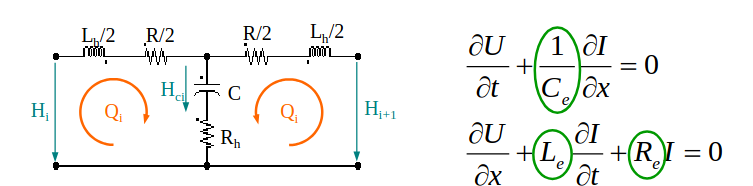
\includegraphics[width=0.5\linewidth]{IMAGES/Hydraulic/Screenshot from 2025-02-21 11-54-39.png}
\end{figure}

A valve can be modeled as a resistor at the end of the circuits and the reservoir as a source. $H_v = \frac{K_v}{2gA_{ref}^2}Q_i^2$ and $R_v(s) = \frac{K_v(s) }{2gA_{ref}^2} \lvert Q_i\rvert$.\\

\subsection{Fundamentals equations}
For a fluid : $A \frac{\partial p}{\partial x} + \tau_o \pi D + \rho g A \sin \alpha + \rho A \frac{DC}{Dt} = 0$ (assume no movement of the pipe and no terms in $dx^2$). With $\tau_o = \frac{\rho \lambda C^2}{8}$ with the Darcy-Weisbach friction coefficient $\lambda$.\\
Then (momentum conservation) : \begin{equation}
    \frac{1}{\rho} \frac{\partial p}{\partial x} + \frac{\partial C}{\partial t} + C \frac{\partial C}{\partial x} + g\sin \alpha + \frac{\lambda \lvert C\rvert C}{2D}=0
\end{equation}

Mass conservation is then : $\frac{1}{\rho} \frac{D\rho}{Dt} + \frac{1}{A} \frac{DA}{Dt} + \frac{\partial C}{\partial x} = 0$. As the fluid has a barotropic behaviour ($\rho = \rho(p)$), with the wave speed : $a_w^2 = \frac{E_w}{\rho} \text{(infinite water medium)} = \frac{1}{\rho(\frac{1}{E_{eau}} + \frac{1}{A} \frac{DA}{Dp})}$ (In a pipe).\\
For a circular pipe (as the constraint in the pipe is : $\sigma = \frac{pD}{2e}$) : \begin{equation}a_w^2 = \frac{1}{\rho (\frac{1}{E_w} + \frac{D}{eE_p})}\end{equation}
Then : \begin{equation}\begin{gathered}
    \frac{Dp}{Dt} + \rho a^2 \frac{\partial C}{\partial x}=0\\
    \frac{Dp}{Dt} = \frac{\partial p}{\partial t} + C \frac{\partial p}{\partial x}\\
    \end{gathered}
\end{equation}
\warning Compressibility of the fluid is hidden in the wave speed. In infinite water media : $a_w = 1430m/s\rvert_{6^\circ C}$ therefore : $E_w = 2.04GPa$. 

Over time, neglect the displacement in the z direction : $\frac{\partial h}{\partial t} = \frac{1}{\rho g} \frac{\partial p}{\partial t}$. As $C<<a$, neglect convective terms : $C\frac{\partial h}{\partial x} << \frac{\partial h}{\partial t}$ and $C\frac{\partial C}{\partial x}<< \frac{\partial C}{\partial t}$.\\

Then : \begin{equation}
    \begin{pmatrix}
        \frac{\partial Q}{\partial t}\\ \frac{\partial h}{\partial t}
    \end{pmatrix} + \begin{pmatrix}
        0 & gA\\ \frac{a^2}{gA} & 0
    \end{pmatrix} \begin{pmatrix}
        \frac{\partial Q}{\partial x} \\ \frac{\partial h}{\partial x}
    \end{pmatrix} = \begin{pmatrix}
        -\frac{\lambda Q \lvert Q\rvert}{2DA}\\ 0
    \end{pmatrix}
\end{equation}
Solution of this system are real and distinct : hyperbolic system. \\

\begin{itemize}
    \item Pressure head : $h_p = \frac{p}{\rho g}$
    \item Kinetic head : $k_k = \frac{C^2}{2g}$
    \item Piezometric head : $h_z = z+h_p$
    \item Energy head : $H = h_z+h_k$
    \item Massic energy : $E = gH$
    \item Lineic friction losses : $\Delta H_r = \lambda \frac{L}{D} \frac{Q \lvert Q\rvert}{2gA_{ref}^2}$
    \item Singular head losses : $\Delta H_r = \frac{K_d}{2gA_{ref}^2} Q \lvert Q\rvert$
\end{itemize}
\warning At any point in the penstock if a hole is drilled, water will rise to $h_z$. In a HQ diagram, the hydraulic circuit characteristic is $z_o-\Delta H_{r,I}^{IV}$. Intersecting point between hydraulic system characteristic and turbine characteristic is the operating point and the net head : $H_b = H_n + \Delta H_{r,I}^{IV}$.\\

Hydraulic power of the turbine : $P_h = \rho g H_n Q$. The efficiency of the turbine is then : $\eta_t = \frac{T\omega}{\rho g H_nQ}$. The electrical power of the tubrine is : $P_{el} = \eta_e P_m = \eta_e \eta_t P_h = \eta_e \eta_t \rho g (H_b-k_r Q^2)Q$, with $k_r$ the global head loss coefficient.\\

\quad \underline{Valve characteristic :}\\
$\Delta H_{r,IV}^V = \frac{K_{dv}(y)}{2gA_{ref}^2} Q^2$. If $y=0$ the valve is closed, 1 is open. Let's $k_v$ be the discharge coefficient (usually $k_v = 0.75$ when the valve is open) such that $k_v = \frac{Q_{eff}}{Q_{theo}}$. $Q_{inj} = k_v(y) A_{ref}^2 \sqrt{2g\Delta H}$ and $\Delta H_{inj} = \frac{k_d(y)}{2gA_{ref}^2}Q^2 \Rightarrow k_d = \frac{1}{k_v^2}$

\begin{figure}[hbt!]
    \centering
    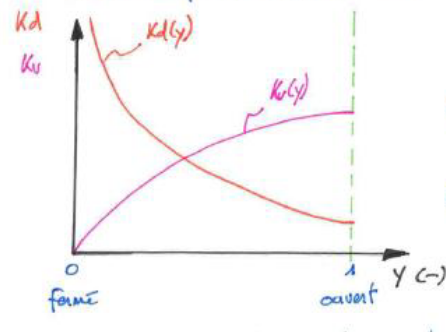
\includegraphics[width=0.6\linewidth]{IMAGES/Hydraulic/Screenshot from 2025-02-28 11-47-55.png}
\end{figure}

The jet velocity : $C_{jet} = 0.98 \sqrt{2g\Delta H}$. 

\subsubsection{Exact solution}
Electrical and hydraulic system share the same equations : $\begin{cases}
    \frac{\partial U}{\partial x}+ L_e' \frac{\partial i}{\partial t} + R_e' i = 0\\ \frac{\partial U}{\partial t} + \frac{1}{C_e'} \frac{\partial i}{\partial x} =0
\end{cases}$; the lineic hydroacoustics capacitance : $C' = \frac{gA}{a^2}[m]$, the lineic hydroacoustic inductance : $L' = \frac{1}{gA} [s^2/m^3]$, the lineic hydroacoustic resistance : $R' = \frac{\lambda \lvert Q \rvert}{2gDA^2} [s/m^3]$.\\

\quad \underline{Wave equation solution :}\\

The wave equations : $\begin{cases}
    \frac{\partial h}{\partial x}+ L' \frac{\partial Q}{\partial t} + R' Q = 0\\ \frac{\partial h}{\partial t} + \frac{1}{C'} \frac{\partial Q}{\partial x} =0
\end{cases}$. Assume complex periodic solution. $\begin{cases}
    \frac{\partial^2\underline{h}}{\partial x^2} = \underline{\gamma}^2 \underline{h}(x)\\
    \frac{\partial^2\underline{Q}}{\partial x^2} = \underline{\gamma}^2 \underline{Q}(x)\\
\end{cases} = \begin{cases}
    \frac{\partial^2\underline{h}}{\partial x^2} = -\frac{\omega^2}{a^2} \underline{h}(x)\\
    \frac{\partial^2\underline{Q}}{\partial x^2} = -\frac{\omega^2}{a^2} \underline{Q}(x)\\
\end{cases}$ (this last relation holds only if conservative system ($R'=0, s=j\omega$) as $\underline{\gamma}^2 = C's(L's+R')$.\\

Let's introduce the characteristic impedance : $\underline{Z}_c = \sqrt{\frac{L's+R'}{C's}}$.\\
The transfer matrix is then : \begin{equation}
    \begin{pmatrix}
        \underline{h}(l)\\ \underline{Q}(l) 
    \end{pmatrix} = \begin{pmatrix}
        \cosh(\underline{\gamma} l) & -\underline{Z}_c \sinh(\underline{\gamma}l)\\
        -\frac{1}{\underline{Z}_c} \sinh(\underline{\gamma}l) & \cosh(\underline{\gamma l})
    \end{pmatrix} \begin{pmatrix}
        \underline{h}(0)\\ \underline{Q}(0)
    \end{pmatrix}
\end{equation}

For conservative system : 
\begin{equation}
    \begin{pmatrix}
        \underline{h}(l)\\ \underline{Q}(l) 
    \end{pmatrix} = \begin{pmatrix}
        \cosh(\frac{\omega l}{a}) & -\underline{Z}_c \sinh(\frac{\omega l}{a})\\
        -\frac{1}{\underline{Z}_c} \sinh(\frac{\omega l}{a}) & \cosh(\frac{\omega l}{a})
    \end{pmatrix} \begin{pmatrix}
        \underline{h}(0)\\ \underline{Q}(0)
    \end{pmatrix}
\end{equation}
With $\underline{\gamma} = \frac{j \omega}{a}$ and $Z_c = \frac{a}{gA}$.\\

The \textbf{global transfer matrix} is then : $[\underline{M}_{tot}] = \Pi [\underline{M}_i]$.\\

\begin{figure}[hbt!]
    \centering
    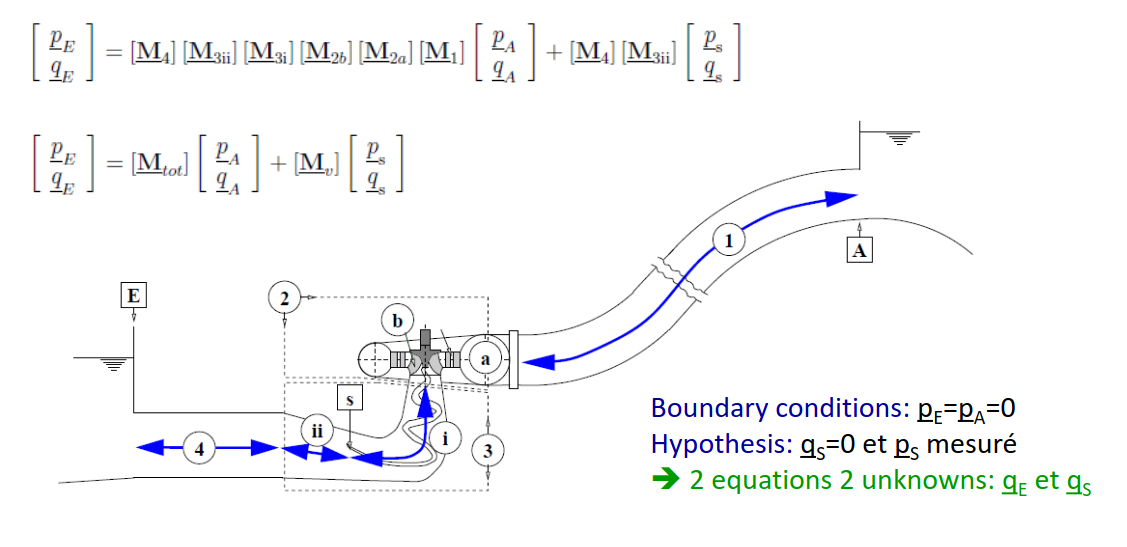
\includegraphics[width=0.5\linewidth]{IMAGES/Hydraulic/Screenshot from 2025-03-07 10-43-44.png}
\end{figure}

\quad \underline{D'Alembert equation solution :}\\
$\begin{cases}
    \frac{\partial^2 Q}{\partial x^2} = C' L' \frac{\partial^2 Q}{\partial^2 t} + C'R' \frac{\partial Q}{\partial t}\\
    \frac{\partial^2 h}{\partial x^2} = C' L' \frac{\partial^2 h}{\partial^2 t} + C'R' \frac{\partial h}{\partial t}\\
\end{cases}$. If conservative : $\begin{cases}
    \frac{\partial^2 Q}{\partial x^2} = \frac{1}{a^2} \frac{\partial^2 Q}{\partial^2 t}\\
    \frac{\partial^2 h}{\partial x^2} = \frac{1}{a^2} \frac{\partial^2 h}{\partial^2 t}\\
\end{cases}$
$h = F_p(t-x/a) + G_r(t+x/a)$, contains progressive wave and retrograde wave.\\

\begin{itemize}
    \item Wave reflection at open-end : $h = 0 \Rightarrow F_p(at) = -G_r(at)$. Reflected wave is the same as incident but in opposite magnitude.
    \item Wave reflection at dead-end : $\frac{\partial h}{\partial x} = 0 \Rightarrow F_p(at) = G_r(at)$. Reflected wave is the same as incident wave.
    \item Wave reflection at junction : $\underline{Z}(x) = \frac{\underline{h}(x)}{\underline{Q}(x)}$, $\underline{h}_t = \underline{h}_i + \underline{h}_r$. There is a junction if there is characteristic impedance change ($Z_c = \frac{a}{gA}$). $\frac{\underline{h}_r}{\underline{h}_i} = \frac{\underline{Z}_{c2}-\underline{Z}_{c1}}{\underline{Z}_{c1} + \underline{Z}_{c2}}$ and $\frac{\underline{h}_t}{\underline{h}_i} = \frac{2 \underline{Z}_{c2}}{\underline{Z}_{c1} + \underline{Z}_{c2}}$.
\end{itemize}

\subsubsection{Water hammer amplitude}
From momentum conservation : $\sum F_x = \int_{V_3} \frac{\partial}{\partial t}(\rho \Vec{C} \cdot \vec{n})dV + \int_{\delta V_3} \rho \vec{C} \cdot(\vec{C} \cdot \vec{n})dA$. From mass conservation : $\frac{dM}{dt}=0$. From both : \begin{equation}
    \Delta p = -\rho a \Delta C \Rightarrow \Delta H = -\frac{a\Delta C}{g}
\end{equation}
For \textbf{full valve closing :} $\Delta C = -C_0$.\\
\begin{itemize}
    \item The travel time (characteristic time) : $t_c = \frac{L}{a}$.
    \item Reflection time : $t_r = \frac{2L}{a}$.
    \item Water hammer period : $T_0 = \frac{4L}{a}$.
\end{itemize}

It is assumed here that the closure time of the valve needs to be smaller than the reflection time; the closure is assumed to be instantaneous. \\
\warning Without losses, it would go on forever. 


\subsubsection{Method : graphical}

\begin{figure}[hbt!]
    \centering
    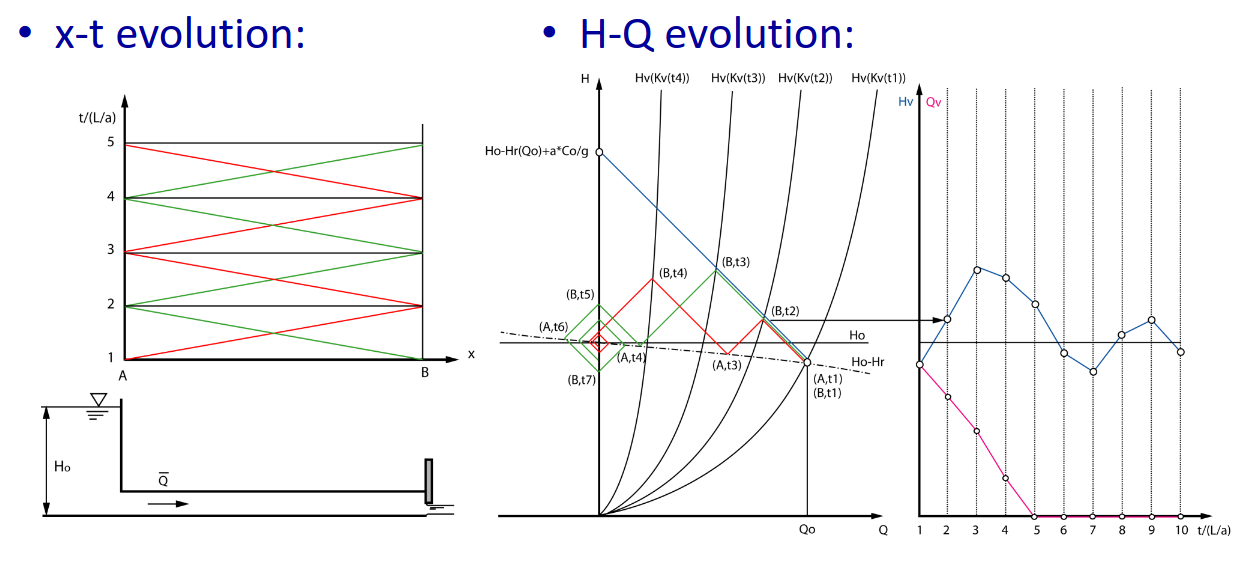
\includegraphics[width=0.5\linewidth]{IMAGES/Hydraulic/Screenshot from 2025-03-14 10-25-28.png}
\end{figure}

\subsubsection{Method : MOC}
Along characteristics line : $Q_p - Q_A + \frac{gA}{a} (H_p-H_A) + \frac{\lambda}{2DA} \Delta t Q_A \lvert Q_A \rvert = 0$ (first order approximation) with $a=-\frac{dx}{dt}$.\\

\subsubsection{Finite difference method}
Equation set : $Q_i^{j+1} = \frac{1}{2} (Q_{i-1}^j  + Q_{i+1}^j) + \frac{1}{2} gA \frac{\Delta t}{\Delta x} (H_{i-1}^j - H_{i+1}^j) - \frac{\lambda }{2DA} \Delta t \overline{ Q}_i \lvert \overline{Q}_i \rvert$, $H_i^{j+1} = \frac{1}{2} \frac{\Delta t}{\Delta x} \frac{a^2}{gA} (Q_{i-1}^j  + Q_{i+1}^j) + \frac{1}{2} (H_{i-1}^j - H_{i+1}^j)$.\\


\begin{figure}[hbt!]
    \centering
    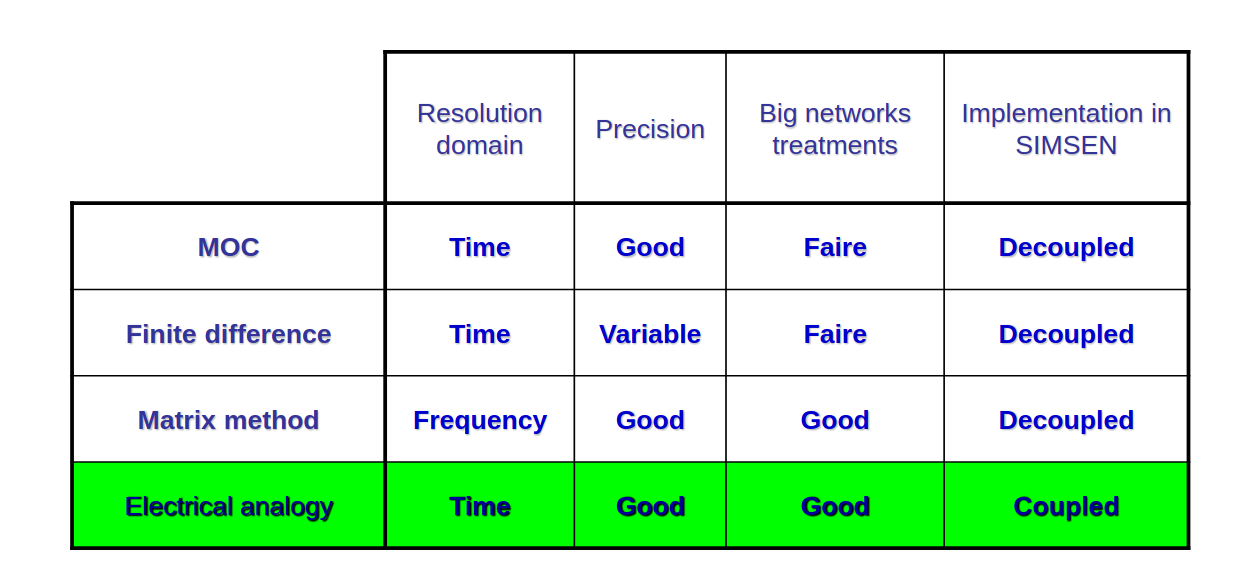
\includegraphics[width=0.5\linewidth]{IMAGES/Hydraulic/Screenshot from 2025-03-14 10-32-40.png}
\end{figure}

\subsection{Water hammer computation}
Full closure of a valve (instantaneous) : $\Delta H = \frac{aC_0}{g}$.\\
If the valve is in the middle of a pipe : high pressure upstream and low pressure downstream (same magnitude, opposite sign). \\

\begin{itemize}
    \item Direct water hammer if $t_{close} < \frac{2L}{a} \Rightarrow \Delta H =\Delta H_{max}= \frac{a C_0}{g} = \frac{aQ_0}{gA}$ 
    \item Reduced water hammer if $t_{close} > \frac{2L}{a} \Rightarrow \frac{\Delta H}{\Delta H_{max}} = \frac{2L/a}{t_{close}}$ \warning Assumes linear decrease of the discharge over time. \begin{equation}
        \Delta H = \frac{2L Q_0}{Ag} \frac{1}{t_{closure}}
    \end{equation} 
\end{itemize}

For Pelton turbines, when injector is closed at $11\%$ we switch from direct water hammer to reduced water hammer and obtain a peak of water hammer amplitude (aka Peak of Michaud).\\

Mitigating measures : amplitude reduction (increase pipe diameter, increase closing time, reduce pipe length), constructive solution (surge tank, pressurized surge tank, additional flywheel for Francis to increase the inertia of the turbine and limit the acceleration, pressure relief valve).\\

Pressure relief valve : reduction of transient overspeed and reduction of water hammer, allows fast guide vane closure ($\simeq 4s$), simultaneous PRV opening, slow PRV closing ($\simeq 20-40s$). 

\begin{figure}[hbt!]
    \centering
    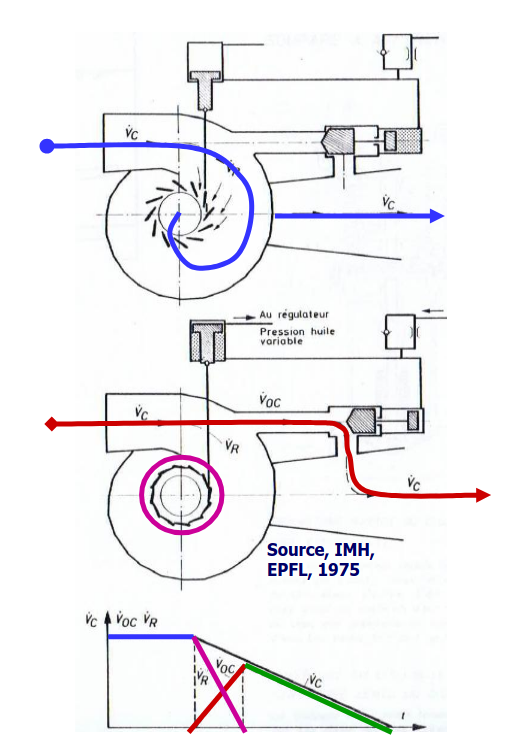
\includegraphics[width=0.7\linewidth]{IMAGES/Hydraulic/Screenshot from 2025-03-14 12-02-39.png}
\end{figure}

From MOC : progressive waves $\begin{cases}
    \frac{dQ}{dt} + \frac{gA}{a} \frac{dh}{dt} + \frac{\lambda Q \lvert Q \rvert}{2DA^2}=0\\ \frac{dx}{dt} = a
\end{cases}$. Then : (progressive wave) $\begin{cases}
    \frac{\Delta h}{\Delta Q} = -\frac{a}{gA}\\ \frac{\Delta x}{\Delta t} = a
\end{cases}$.\\
\warning Retrograde waves imply $-a$\\

\begin{figure}[hbt!]
    \centering
    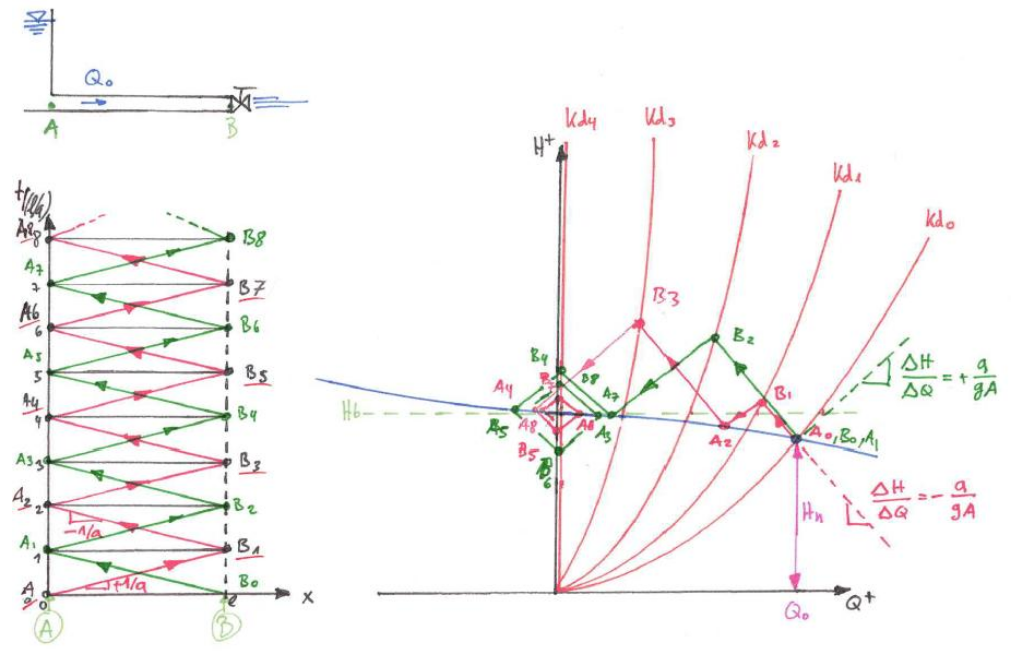
\includegraphics[width=0.7\linewidth]{IMAGES/Hydraulic/Screenshot from 2025-03-21 11-50-24.png}
\end{figure}

\begin{figure}[hbt!]
    \centering
    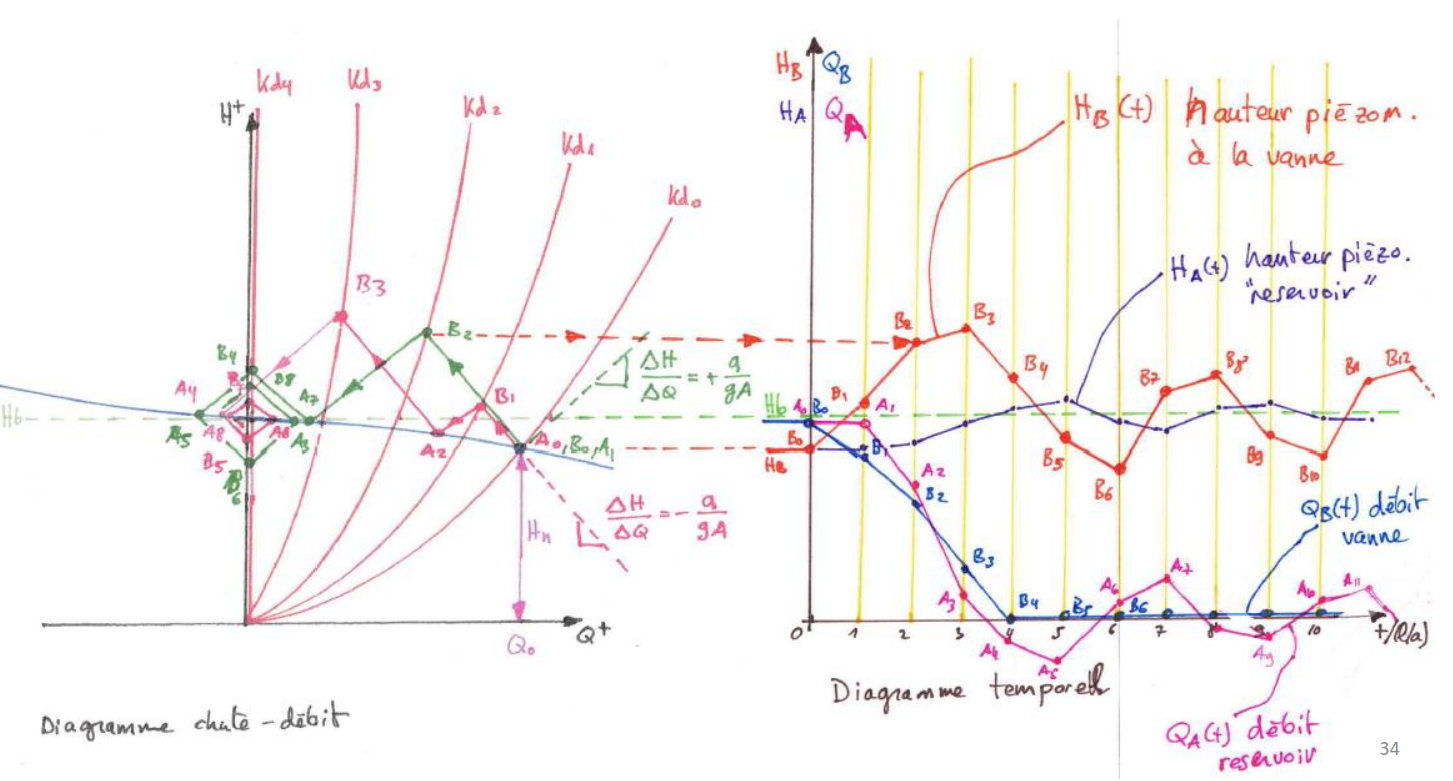
\includegraphics[width=0.7\linewidth]{IMAGES/Hydraulic/Screenshot from 2025-03-21 11-51-32.png}
\end{figure}

In case of multiple length, diameter, friction in series : use equivalent pipes! \begin{itemize}
    \item $L_{tot} = \sum l_i$
    \item $t_{tot} = \sum \frac{l_i}{a_i} \Rightarrow a_{tot} = \frac{l_{tot}}{t_{tot}}$
    \item $A_{eq} = \frac{l_{tot}}{\sum \frac{l_i}{A_i}} \Rightarrow D_{eq} = \sqrt{\frac{l_{tot}}{\sum \frac{l_i}{D_i^2}}}$
    \item $\lambda_{eq} = \frac{D_{eq}A_{eq}^2}{l_{tot}} \sum \frac{\lambda_i l_i}{D_i A_i^2}$
\end{itemize}

\subsection{Electrical analogy}
We have the equations : $\begin{cases}
    \frac{\partial h}{\partial x} + L' \frac{\partial Q}{\partial t} + R' Q = 0\\
    \frac{\partial h}{\partial t} + \frac{1}{C'} \frac{\partial Q}{\partial x} = 0\\
\end{cases}$. Then : \begin{equation}
\begin{gathered}
    \begin{pmatrix}
        C & 0&0\\0 & L/2 &0\\0 & 0 & L/2
    \end{pmatrix} \frac{d}{dt} \begin{pmatrix}
        h_{i+1/2}\\Q_i\\ Q_{i+1}
    \end{pmatrix} + \begin{pmatrix}
        0&-1&1\\1&R/2&0\\
        -1&0&R/2
    \end{pmatrix} \begin{pmatrix}
        h_{i+1/2}\\Q_i\\ Q_{i+1}
    \end{pmatrix} = \begin{pmatrix}
        0\\ h_i\\-h_{i+1}
    \end{pmatrix}\\
    A\frac{d}{dt}X + B(X)X = C
    \end{gathered}
\end{equation}

With $\begin{cases}
    R = R'dx\\ L = L'dx\\ C=C'dx
\end{cases}$ and $\begin{cases}
    C=  \frac{dx g A}{a^2} [m^2]\\
    L = \frac{dx}{gA} [s^2/m^2]\\
    R = \frac{\lambda dx \lvert Q \rvert }{2gDA^2}[s/m^2]\\
\end{cases}$
\warning Head is computed in the middle of the control volume while discharge is computed at the ends.\\

\begin{figure}[hbt!]
    \centering
    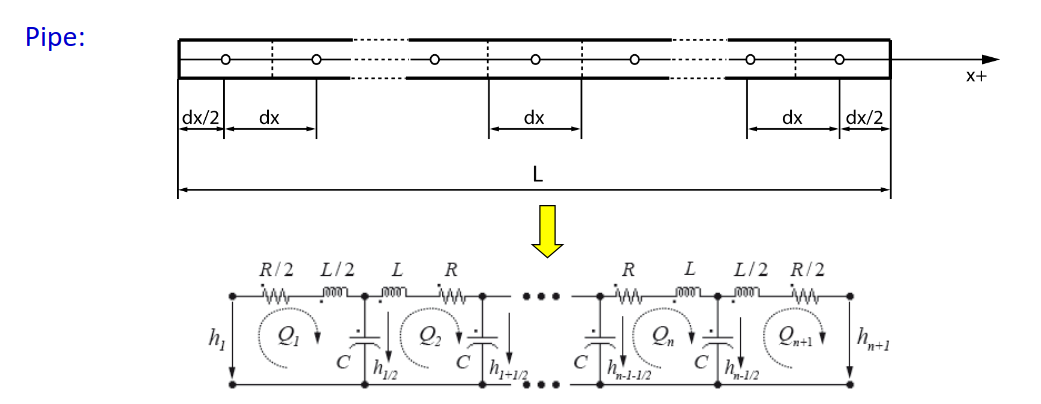
\includegraphics[width=0.5\linewidth]{IMAGES/Hydraulic/Screenshot from 2025-03-28 11-38-27.png}
\end{figure}

For a general system : \begin{figure}[hbt!]
    \centering
    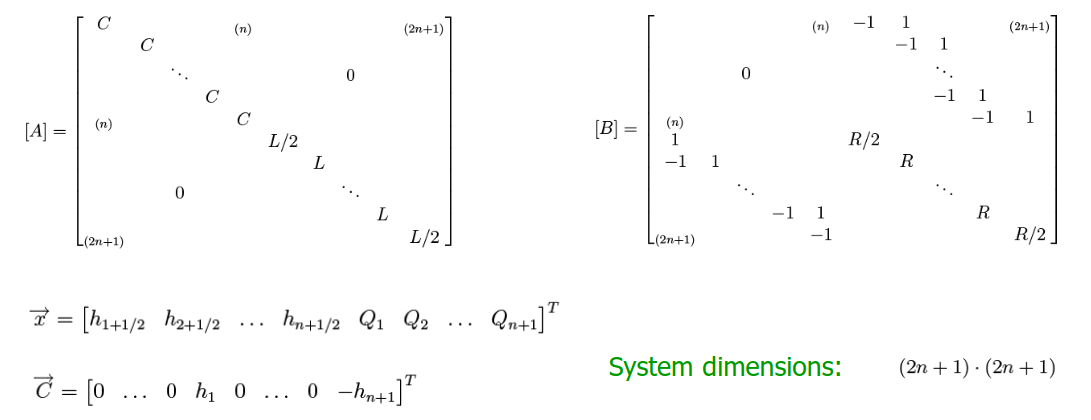
\includegraphics[width=0.5\linewidth]{IMAGES/Hydraulic/Screenshot from 2025-04-04 10-25-42.png}
\end{figure}

The first order explicit method is such that : $[A] \frac{x^{j+1} - x^j}{\Delta t} + [B(x^j)] x^j = c \Rightarrow x^{j+1} = x^j + [A]^{-1} (c-[B(x^j)] x^j)\Delta t$. \warning The integration step needs to be : $dt < \frac{dx}{a}$ (CFL criteria). The Courant number is then : $C_r = \frac{a dt}{dx}\leq 1$.\\

Different cases :
\begin{itemize}
    \item Steady-state : terms in $\frac{d}{dt} = 0$, $H_1-H_2 = \frac{R}{2}Q_1 + \frac{R}{2}Q_2 = RQ_1$
    \item If $H_2$ increases then $Q_2$ decreases : $h_{c1}-H_2\simeq \frac{L}{2} \frac{dQ_2}{dt}<0$
    \item If $Q_2$ decreases, $h_{c1}$ increases : $C\frac{dh_{c1}}{dt} = Q_1-Q_2>0$
\end{itemize}

Error measurement : if $\frac{\lambda}{dx} = 10 \Rightarrow e<3\%$, if $\frac{\lambda}{dx} = 20 \Rightarrow e<1\%$ ($a = \lambda f$). This gives the number of elements needed ($L_{pipe}/dx$)/the length of each element.\\

Other method : selection of time basis dT : selection of dT (usually 0.01s), computation of wave speed a, computation of the element length, adaptation of wave speed a to have positive integer number of elements. \\

\subsection{Modeling of hydraulic components}

\begin{figure}[hbt!]
    \centering
    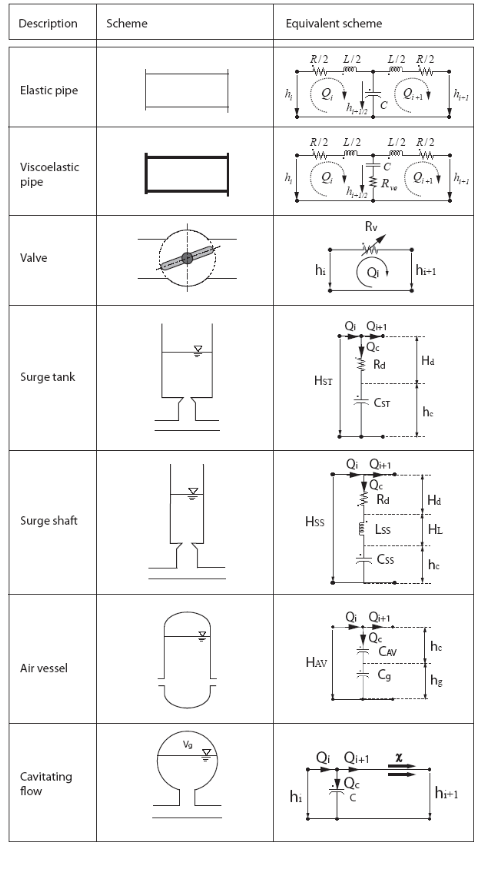
\includegraphics[width=0.5\linewidth]{IMAGES/Hydraulic/Screenshot from 2025-04-04 11-52-17.png}
\end{figure}

\begin{itemize}
    \item Viscoelastic pipe : viscoelasticity from pipe mx ($\sigma = E_{pipe} \varepsilon + \mu_{pipe}\frac{d\varepsilon}{dt}$) or fluid ($\frac{dp}{dt} = \frac{E_{fluid}}{\rho} \frac{d\rho}{dt} + \frac{\mu_{fluid}}{\rho} \frac{d^2 \rho}{dt^2}$).
    \item Valve : $Q = K_v A_{ref} \sqrt{2g dH_r}$, $dH_r = \frac{K_d(y)}{2gA_{ref}^2} \lvert Q \rvert Q$ \warning It is better to use discharge coefficient $K_d$ and assume linear behavior.
    \item Surge tank : volume $\frac{dV_{st}}{dt} = A(z) \frac{dz}{dt} \Rightarrow A(z) \frac{d h_c}{dt} = Q_c$, losses $H_d = \frac{K_d}{2gA_{ref}^2} Q_c^2$, inertia $L_{ss} = \frac{h_c-Z_{min}}{gA}$, equivalent scheme $C_{st} = A(Z)$ and $R_d(Q_c) = \frac{K_d}{2gA_{ref}^2} \lvert Q_c \rvert$, the inductance is directly the inertia (usually neglected).
\end{itemize}



\end{document}